\documentclass{article}
\usepackage{amsmath}
\usepackage{amssymb}
\usepackage[pdftex]{graphicx}
\usepackage[framed,numbered,autolinebreaks,useliterate]{mcode}
\lstset{breakatwhitespace=false}

\pdfpagewidth 8.5in
\pdfpageheight 11in
\topmargin -1in
\headheight 0in
\headsep 0in
\textheight 8.5in
\textwidth 6.5in
\oddsidemargin 0in
\evensidemargin 0in
\headheight 50pt
\headsep 0in
\footskip .75in

\title{STA 601 - Homework 10}
\author{Kedar Prabhudesai}
\date{October 18, 2013}

\begin{document}
\maketitle

\noindent {\Large\underline{\textbf{Logistic Regression Model:}}}\\

Likelihood,\\

$L(y \mid x,\beta) = \prod_{i=1}^{n}{\left(\frac{1}{1+e^{-x_i'\beta}}\right)^{y_i}\left(\frac{1}{1+e^{x_i'\beta}}\right)^{1-y_i}}$\\
$\therefore log[L(y \mid x,\beta)] = \sum_{i=1}^{n}{\left[y_i log\left(\frac{1}{1+e^{-x_i'\beta}}\right) + (1-y_i)log\left(\frac{1}{1+e^{x_i'\beta}}\right)\right]}$

Priors,\\
$\left(\beta_0,\beta_1,\ldots,\beta_p\right) \sim \mathcal{N}_p(\mu_p,\Sigma_p)$. $p$-Variate Normal Distribution.\\

\noindent {\Large\underline{\textbf{Metropolis-Hastings Algorithm:}}}\\

We update each $\beta_i$ as follows:\\

\begin{itemize}
\item Draw, $\beta_i^* \sim \mathcal{N}(\beta_i^{(s)},5).$
\item Compute, $r = log[L(y \mid x,\beta_i^*,\beta_j^{(s)})] + log[\pi(\beta_i^*,\beta_j^{(s)})] - log[L(y \mid x,\beta_j^{(s)})] - log[\pi(\beta_j^{(s)})]$, where, $j$ represents all coefficients other than $i$.
\item Accept, $\beta_i^{(s+1)} = \beta_i^*$ with probability$\left(1,min(r)\right)$.\\
\end{itemize}

\noindent {\Large\underline{\textbf{Results:}}}\\

\begin{center}
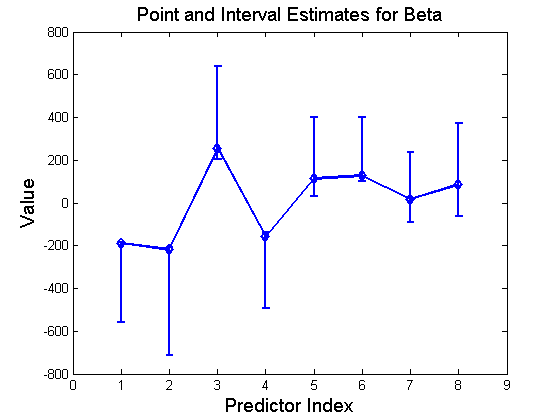
\includegraphics[scale=0.5]{BetaResults.png}\\
\end{center}

\pagebreak
\noindent {\Large\underline{\textbf{Appendix:}}}\\
\lstinputlisting{C:/Users/ksp6/Documents/Classes/2013-Fall/STA601-BayesAndModStats/homeworks/hw10/hw10.m}

\end{document}